\documentclass{report}
\usepackage{graphicx}
\usepackage{hyperref}
\usepackage{geometry}
\usepackage{tabularx}
\usepackage{float}


% Packages
% Add any additional packages you need here

% Document information
\title{Your Thesis Title}
\author{Your Name}
\date{\today}

\geometry{
    a4paper,
    left=30mm,
    right=30mm,
    top=30mm,
    bottom=30mm
}

\begin{document}

% Title page
\maketitle

% Abstract
\begin{abstract}
% Add your abstract here
\end{abstract}

% Table of contents
\tableofcontents

% Chapters
\chapter{Introduction}
In recent years, the restaurant industry has experienced a significant shift towards digitization. The move towards web-based restaurant management applications signifies a critical step in this direction, offering a bridge between the traditional dining experience and modern technological conveniences. This final year project aims to design, develop, and evaluate a sophisticated web-based restaurant management application, leveraging contemporary web technologies to enrich the dining experience for customers and streamline restaurant operations.

The application at the core of this project is built upon a React.js frontend and a Django backend, handled by a SQLite database. The decision to use React.js stems from its efficiency in rendering dynamic user interfaces and facilitating an interactive web experience. Django offers comprehensive support for web development needs, including ORM (Object-Relational Mapping) for database interactions, REST Framework for API development, and built-in mechanisms for user authentication and authorization.

One of the application's standout features is its use of QR codes, enabling customers to access the menu and place orders directly from their smartphones. This not only enhances the dining experience by offering convenience and speed but also aligns with contemporary expectations for contactless services. The application further personalizes the customer experience through algorithms that analyze user preferences and order history, delivering tailored menu recommendations that cater to individual tastes and dietary needs. This implementation also solves the problem of splitting bills by introducing a session system to tables which allows customers to order under their own bill or share the bill with others easily all while sitting at the same table.

The backend architecture of the restaurant management system is designed to be efficient. The Django ORM facilitates interactions with the database, abstracting SQL queries into Python. Django REST Framework (DRF) plays a crucial role in this architecture, providing tools for building a RESTful API that the React frontend consumes. This API layer enables seamless communication between the frontend and backend, ensuring that data flows securely and efficiently across the application.

On the frontend, React.js's component-based architecture allows for the development of a modular and interactive user interface. The use of React components enables the reuse of UI elements across the application, ensuring consistency and reducing development time. State management is handled adeptly through React's context API, facilitating the tracking and updating of application state across components without prop drilling. This is crucial for managing user sessions, order details, and authentication states throughout the application. Additionally, the application employs React Router for client-side routing, enhancing the user experience with smooth transitions between views without the need for page reloads.

The database architecture is designed to cater to the needs of restaurant management. It includes models for the restaurant settings, menu items, orders, and customer profiles, among others. Each model is designed to capture data and relationships, enabling the application to offer features such as menu customization, order tracking, and personalized recommendations.

An integral part of the project is the implementation of a recommender algorithm within the UserProfile model. This algorithm is a cornerstone of the application's ability to offer personalized menu recommendations, to enhance the customer experience. By analyzing user preferences and order history, the algorithm identifies preferences, suggesting menu items that align with the user's taste profile. The decision to use a hybrid filtering approach, combining the strengths of collaborative and content-based filtering, underscores the project's commitment to leveraging advanced technologies for personalization.

For restaurant staff, the project includes features for order tracking, menu management, and sales analysis. These tools are designed to improve operational efficiency, enabling staff to manage orders more effectively, update the menu as needed, and analyze sales data to make informed decisions. The inclusion of a kitchen display system further streamlines kitchen operations, displaying orders in real-time and helping staff prioritize based on urgency.

In conclusion, this final year project aims to further improve current implementations and cover some gaps that have not been done before such as the recommender system and the session system.

\chapter{Literature Review}
\section{Evolution of Restaurant Management Systems}
The evolution of restaurant management systems has seen a shift from traditional paper-based methods to digital systems, driven by the need for improved efficiency and customer experience. Traditional systems, such as paper-based menu cards and manual order taking, have limitations in terms of time consumption, manual errors, and customer dissatisfaction \cite{1}. The adoption of digital systems, such as tablet food ordering and digital based ordering, has aimed to address these limitations by providing cost and time efficiency benefits for both management and customers \cite{1}.
Factors driving the adoption of digital restaurant management systems include the need for faster services, reduced dependency on waiters, which increases productivity \cite{3}. Additionally, the use of technology to replace some of the jobs done by human beings and make machines do the work has been a driving factor in the adoption of online food ordering management systems \cite{4}.

The adoption of digital systems has also been influenced by the increasing trend of consumers adopting a more tech-savvy approach to conducting business transactions and leisure activities, leading to the need for restaurant owners to keep up with technological advancements to attract and retain a broader customer base \cite{5}.
Overall, the evolution of restaurant management systems from traditional to digital has been driven by the need for improved efficiency, reduced manual errors, and enhanced customer satisfaction, while also aligning with the changing technological landscape and consumer preferences.

\section{Digital Ordering Systems}
The implementation of digital ordering systems in restaurants has been shown to have a significant impact on customer experience and business outcomes. The use of QR codes for ordering has been designed to provide more advantages, including electronic payment of bills and entertainment facilities, and to reduce the time between ordering and delivering goods to customers \cite{6}. The system allows customers to place food orders by scanning the QR code on the restaurant table, which then directs them to a digital version of the restaurant's menu, enabling them to place orders directly from their phones \cite{2}. This automation of the ordering process has been found to reduce the time of order registry to delivery, improving customer satisfaction and business efficiency \cite{6}.
The use of digital menus in restaurants has been shown to provide several benefits, including the elimination of traditional ordering stages, more favourable choices for customers, and the ability to pay bills digitally, which prevents the pollution of money exchange and has a significant effect on protecting the environment due to the reduced use of paper \cite{6}. The system also allows restaurant owners to have an insightful view of their business data, such as sales data, which can improve decision-making and forecasting demand using data analysis techniques \cite{2}.

Research has shown that the implementation of digital ordering systems has led to increased customer satisfaction, improved table turnover, and reduced labour and menu costs \cite{5}. Customers have reported that the QR menu ordering systems provide convenience, value, and enjoyment, leading to increased customer attraction and satisfaction \cite{5}. Furthermore, the system has been found to improve table turnover and reduce labour and menu costs, leading to improved business efficiency \cite{5}.
In conclusion, the implementation of QR code ordering systems in restaurants has had a positive impact on customer experience and business outcomes, leading to improved customer satisfaction, business efficiency, and insightful views of business data for restaurant owners.

\section{Customer Behavior and Technology Acceptance Towards Digitalisation}
The Unified Theory of Acceptance and Use of Technology (UTAUT) model has been applied to understand customer willingness to use QR code ordering systems in luxury restaurants in Xi'an, China \cite{5}. The UTAUT model contains four independent variables: performance expectancy, effort expectancy, social influence, and facilitating conditions 1.2. Additionally, the UTAUT 2 model, an extended version of UTAUT, includes hedonic motivation, price value, trust, experience, and habit as independent variables, focusing more on the individual use of technology \cite{5}. The study found that performance expectancy, effort expectancy, social influence, facilitating conditions, hedonic motivation, price value, and trust positively affect customer intention to use QR menu ordering \cite{5}. However, effort expectancy and facilitating conditions negatively affect customer behavioural intention \cite{5}.

Factors influencing customer behaviour and acceptance include performance expectancy (the degree to which technology will benefit consumers performing certain activities), effort expectancy (the degree of ease associated with consumers' use of technology), social influence, facilitating conditions, hedonic motivation, price value, and trust \cite{5}. These factors have been found to significantly influence customers' behavioural intention to use QR menu ordering systems \cite{5}.

Moreover, the study revealed that trust is an important variable affecting customers' behavioural intention to use the QR menu, especially when they are asked to provide confidential information such as transaction codes or personal details \cite{5}. This highlights the significance of trust in influencing customer acceptance of QR code ordering systems.

\section{Challenges and Solutions}
The operational challenges faced by restaurants in implementing and managing web-based systems include difficulties in managing customer orders during peak hours, the need for efficient labour scheduling, and the management of customer reservations and waitlists \cite{7}. 

Potential solutions to these challenges involve the implementation of a self-ordering System, which can automate the ordering process, provide real-time order tracking, and manage customer reservations efficiently \cite{7}.

Common technological barriers in implementing web-based systems include compatibility issues with existing systems, scalability concerns, and the need for secure data exchange between different systems \cite{2}.

These barriers can be overcome by using open-source technologies to maintain low costs, ensuring that the system is scalable to accommodate many users, and implementing secure data exchange protocols to protect customer and business data \cite{2}. 

\section{Current Implementations}
There are some QR code ordering solutions reviewed, including solutions such as Toast \cite{8}, Square \cite{9}, Zuppler \cite{10}, TouchBistro \cite{11}, Bbot \cite{12}, Menufy \cite{13}, and Future Ordering \cite{14}. These solutions provide a a lot of functionalities, such as online ordering, and loyalty programs, to specialized tools for creating and managing QR code-based menus. To summarise it, each solution presents features such as real-time menu updates, and data analytics. These solutions highlights the importance of selecting a system that aligns with a restaurant's specific operational needs, budget, and customer engagement goals, emphasizing the role of digital technology in transforming the traditional dining model into a more interactive, convenient, and streamlined process.

Future Ordering \cite{14} is one of the most notable solutions in the UK as several big restaurant names such as KFC, Nandos and Burger King have implemented them. Future Ordering provides a digital ordering platform for food and beverage businesses, focusing on app, web, and kiosk channels. Their system supports various user journeys, including curbside, click’n’collect, and table ordering, and offers comprehensive management tools for digital channels. However, Future Ordering requires you to have their proprietary hardware which can be a barrier in terms of cost for smaller restaurants.
\begin{table}[H]
    \centering
    \begin{tabularx}{\textwidth}{|X|c|c|c|c|}
    \hline
    \textbf{Solution} & \textbf{Online Ordering} & \textbf{Customer Analysis} & \textbf{Data Analytics} & \textbf{Personalised Experience} \\
    \hline
    Toast \cite{8} & Yes & No & Yes & No \\
    \hline
    Square \cite{9} & Yes & Yes & Yes & No \\
    \hline
    Zuppler \cite{10} & Yes/No & No & Yes & No \\
    \hline
    TouchBistro \cite{11} & No & No & Yes & No \\
    \hline
    Bbot \cite{12} & Yes & No & Yes & No \\
    \hline
    Menufy \cite{13} & Yes & No & Yes & No \\
    \hline
    Future Ordering \cite{14} & Yes & No & Yes & No \\
    \hline
    \end{tabularx}
    \caption{Comparison of QR code ordering solutions}
    \label{tab:comparison}
\end{table}

\section{Research Gaps}

While the adoption of digital ordering systems and the implementation of technologies like QR codes have greatly improved the efficiency of order-taking and the overall customer experience, there is a significant gap regarding personalized customer experiences through these digital systems. Most existing systems, as discussed, focus on streamlining operations, reducing errors, improving table turnover, and providing insights into business data. However, there's a scarcity of discussion around how these systems can leverage customer data to offer personalized dining experiences. 

Personalization in restaurant management systems can significantly enhance customer satisfaction and loyalty by making customers feel valued and understood. By tracking previous orders and preferences, restaurants can offer tailored recommendations, which not only improves the customer experience but can save time during ordering as the recommendations are more likely to be accepted.

Another gap is the lack of solution for bill splitting. Bill splitting is a common issue in restaurants, especially when dining in groups. It can be a time-consuming and error-prone process for both customers and staff. A digital ordering system that can automate the bill splitting process can significantly improve the customer experience and reduce the workload on staff.

\section{Conclusion}
To conclude this literature review, the evolution of restaurant management systems has seen a shift from traditional paper-based methods to digital systems, driven by the need for improved efficiency and customer experience. The adoption of digital systems has been influenced by the increasing trend of consumers adopting a more tech-savvy approach to conducting business transactions and leisure activities, leading to the need for restaurant owners to keep up with technological advancements to attract and retain a broader customer base. 

The implementation of digital ordering systems in restaurants has been shown to have a significant impact on customer experience and business outcomes, leading to improved customer satisfaction, business efficiency, and insightful views of business data for restaurant owners. The Unified Theory of Acceptance and Use of Technology (UTAUT) model has been applied to understand customer willingness to use QR code ordering systems in luxury restaurants in Xi'an, China [5]. Factors influencing customer behaviour and acceptance include performance expectancy, effort expectancy, social influence, facilitating conditions, hedonic motivation, price value, and trust. These factors have been found to significantly influence customers' behavioural intention to use QR menu ordering systems.

The operational challenges faced by restaurants in implementing and managing web-based systems include difficulties in managing customer orders during peak hours, the need for efficient labour scheduling, and the management of customer reservations and waitlists. Common technological barriers in implementing web-based systems include compatibility issues with existing systems, scalability concerns, and the need for secure data exchange between different systems.

There are some QR code ordering solutions reviewed, including solutions such as Toast, Square, Zuppler, TouchBistro, Bbot, Menufy, and Future Ordering. These solutions provide a lot of functionalities, such as online ordering, and loyalty programs, to specialized tools for creating and managing QR code-based menus. 

However, there is a significant gap regarding personalized customer experiences through these digital systems and the lack of solution for bill splitting. Personalization in restaurant management systems can significantly enhance customer satisfaction and loyalty by making customers feel valued and understood. By tracking previous orders and preferences, restaurants can offer tailored recommendations, which not only improves the customer experience but can save time during ordering as the recommendations are more likely to be accepted. A digital ordering system that can automate the bill splitting process can significantly improve the customer experience and reduce the workload on staff. This research aims to address these gaps by proposing a digital ordering system that leverages customer data to offer personalized dining experiences and automate the bill splitting process. The next chapter will discuss the research methodology used to achieve this goal.




\chapter{Methodology}
\section{Overview}
This chapter outlines the systematic methodology employed to design, develop, and evaluate a web-based restaurant management application. The application leverages modern web technologies, including a React.js frontend, to enhance the dining experience by enabling customers to place orders using QR codes, receive personalized menu recommendations, and choose flexible bill-sharing options. The development process is guided by user-centered design principles, aiming to improve customer satisfaction and operational efficiency for restaurants.

\section{System Design}
The web application is built using React.js frontend paired with Django backend, with a SQLite database. The frontend is responsible for rendering the user interface and handling user interactions, while the backend manages the business logic and data storage. The frontend and backend communicate via Djano RESTful APIs using Axios from React, enabling the application to be scalable and maintainable. The application can hosted on a cloud platform, such as AWS or Heroku or Railway.

\subsection{Backend Architecture}
\begin{itemize}
    \item \textbf{Models}: Django models define the database schema. Each model corresponds to a database table and is used for creating, retrieving, updating, and deleting records. For instance, models like Place, Category, MenuItem, and Order represent the core entities of the restaurant management system.
    \item \textbf{Views}: Django views handle the business logic of the application. They receive web requests and return web responses. Views interact with models and return JSON responses (in the case of a REST API used by a React frontend).
    \item \textbf{URL Routing}: Django's URL routes incoming requests to the appropriate view based on the request URL. This is where you define URL patterns for your API endpoints.
    \item \textbf{Django REST Framework}: For integrating with a React frontend, Django REST Framework (DRF) is used to build a RESTful API. DRF provides serializers for converting complex data types to and from JSON and viewsets for handling common API operations.
    \item \textbf{Authentication and Authorization}: Django comes with a built-in authentication system, and DRF offers additional mechanisms for API authentication, such as token authentication.
    \item \textbf{Database}: Django supports various databases like PostgreSQL, MySQL, SQLite, and Oracle. However, SQLite was chosen for its simplicity and ease of use.
\end{itemize}

\subsection{Frontend Architecture}
\begin{itemize}
    \item \textbf{React Components}: The frontend is built using React.js. React components are used to create reusable UI elements, such as buttons, forms, and menus.
    \item \textbf{State Management}: React's state and context API are used to manage the application's state, such as user authentication, order details, and session information.
    \item \textbf{Routing}: React Router is used for client-side routing, allowing the application to navigate between different views without a page refresh.
    \item \textbf{API Integration}: Axios is used to make HTTP requests to the Django backend, enabling the frontend to fetch and send data to the server.
    \item \textbf{User Interface}: The frontend is designed to be responsive and user-friendly, with a focus on providing an intuitive and visually appealing experience for customers.
    \item \textbf{Bulma SCSS}: On top of using React Components, additional Bulma SCSS components were used to style the application, this allows the application to be responsive and have uniform styling.
\end{itemize}

\section{Database Architecture}
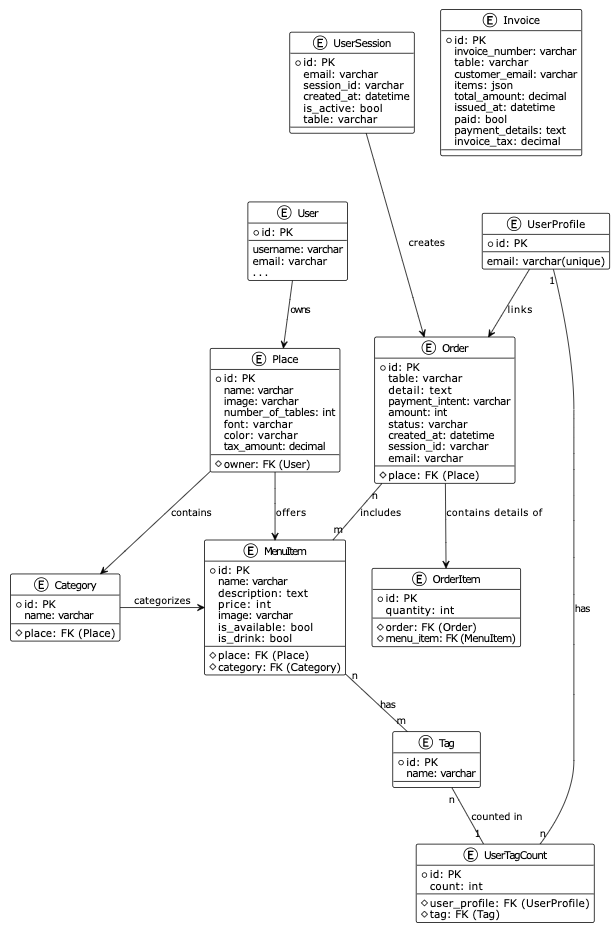
\includegraphics[width=1\textwidth]{images/databasediagram.png}

\subsection{Place}
Represents a restaurant or place that uses the app. It includes details like the owner (linked to the Django \texttt{User} model), name, image, number of tables, and aesthetic customizations (font and color). A new field, \texttt{tax\_amount}, has been added to manage tax calculations.

\subsection{Category}
Organizes menu items into categories (e.g., appetizers, entrees, desserts) for each place. This helps in structuring the menu for easier navigation by the customers.

\subsection{MenuItem}
Details about each menu item, including the place it belongs to, its category, name, description, price, and availability. It also specifies whether the item is a drink and allows for tagging (e.g., vegan, spicy) through a many-to-many relationship with the \texttt{Tag} model.

\subsection{Tag}
Used to label menu items with specific attributes, enhancing the ability to offer personalized recommendations based on customer preferences.

\subsection{UserSession}
Tracks active sessions by customers, including their email, session ID, and table number. It supports functionalities like order tracking and session management.

\subsection{Order}
Records details of customer orders, including the items ordered (linked through \texttt{OrderItem}), the table and place, payment information, and status. It also tracks the session and customer email.

\subsection{OrderItem}
A through model for the many-to-many relationship between \texttt{Order} and \texttt{MenuItem}, capturing the quantity of each menu item ordered.

\subsection{Invoice}
Manages billing information, including the items ordered, total amount, and payment status. It introduces the \texttt{items} field as a JSON structure to store ordered items, allowing for flexible representation of order details.

\subsection{UserProfile}
Represents a user's profile with a unique email. It is linked to \texttt{Tag} through \texttt{UserTagCount} to track preference metrics.

\subsection{UserTagCount}
Tracks the count of tags associated with a user's orders, facilitating the personalization engine to recommend items based on preferred tags.

% \section{Personalization and Recommendations}
% The schema supports advanced personalization features:
% \begin{itemize}
%     \item \textbf{Personalized Menu Recommendations:} By analyzing a user's order history and preferences (e.g., most ordered tags, preferred price range), the system can recommend menu items that match their taste. This is achieved through methods in the \texttt{UserProfile} model, which calculate preferences based on past orders and tag popularity.
%     \item \textbf{Recommendation Algorithms:} The application uses detailed methods within \texttt{UserProfile} to recommend not only individual food and drink items but also combo meals by creating all possible combinations of recommended food and drink items.
% \end{itemize}

% \section{Key Features and Relationships}
% \begin{itemize}
%     \item The system uses Django's built-in \texttt{User} model for authentication and ownership, linking restaurant places directly to user accounts.
%     \item The \texttt{ForeignKey} and \texttt{ManyToManyField} relationships are utilized extensively to create a network of interconnected entities, enabling complex queries for personalization, order tracking, and session management.
%     \item The application's database design is geared towards enhancing the user experience through features like personalized recommendations, flexible ordering sessions, and detailed order and billing management.
%     \item The use of methods like \texttt{create\_session\_for\_email} in \texttt{UserSession} and recommendation algorithms in \texttt{UserProfile} demonstrate the application's dynamic and user-focused functionality.
% \end{itemize}
% This architecture facilitates a rich, interactive, and personalized user experience in the restaurant management domain, blending traditional e-commerce models with innovative features tailored to the hospitality industry.

\section {Digital Menu Implementation}
QR codes placed on each table serve as the entry point for customers to access the menu and place orders. Upon scanning the QR code with a smartphone, customers are directed to a web interface where they can browse the menu, make selections, and specify their order preferences.
\subsection{Menu Display}
The menu is organized into categories, with each item displaying its name, description, price, and availability. The user interface is designed to be visually appealing and easy to navigate, with a responsive layout that adapts to different screen sizes.
\subsection{Order Placement}
Customers can add items to their order by clicking on the menu items and specifying the quantity. The system tracks the items ordered and the customer's session, allowing for order tracking and billing.
\subsection{Personalized Recommendations}
The application uses the customer's order history and preferences to recommend menu items that match their taste. This is achieved through methods in the \texttt{UserProfile} model, which calculate preferences based on past orders and tag popularity. The algorithm takes into account the most ordered tags and preferred price range to recommend items that align with the customer's preferences.

\section{Recommendation Algorithm}
The recommendation algorithm embedded within the \texttt{UserProfile} model of our restaurant management application is designed to offer personalized menu suggestions to users. It analyzes users' past orders, preferences, and price sensitivity to recommend items that align with their tastes.

\subsection{User Preferences and Order History Analysis}
\begin{itemize}
    \item The algorithm commences by evaluating the user's previous orders to deduce preferences. This involves:
    \begin{itemize}
        \item Calculating the average price of the items ordered to establish a preferred price range.
        \item Identifying the most ordered tags to understand the user's food preferences.
    \end{itemize}
\end{itemize}

\subsection{Tag-Based Recommendations}

\begin{itemize}
    \item Users are linked to tags via the \texttt{UserTagCount} model, reflecting their taste preferences.
    \item Menu items are scored based on their relevance to the user's preferred tags, with higher scores for better-matched items.
\end{itemize}

\subsection{Price Sensitivity}

\begin{itemize}
    \item The algorithm adjusts scores for items within the user's preferred price range, favoring those that align with past spending habits.
\end{itemize}

\subsection{Personalized Recommendations}

\begin{itemize}
    \item For food items: Excludes drinks, scoring food items based on tag preferences and price sensitivity.
    \item For drink items: Similar process, but focuses solely on beverages, tailoring recommendations accordingly.
\end{itemize}

\subsection{Combining Recommendations for Combo Meals}

\begin{itemize}
    \item Creates combo meal suggestions by pairing the  top food and drink recommendations.
\end{itemize}

\subsection{Example Usage}
\subsection*{Step 1: Determining the Preferred Price Range}

Assume the user has ordered the following items:

\begin{itemize}
    \item Pizza: \$12 (Quantity: 2)
    \item Burger: \$9 (Quantity: 1)
    \item Salad: \$7 (Quantity: 3)
\end{itemize}

\subsection*{Calculation}

\begin{verbatim}
Total spent on Pizza = $12 * 2 = $24
Total spent on Burger = $9 * 1 = $9
Total spent on Salad = $7 * 3 = $21

Total spent = $24 + $9 + $21 = $54
Total quantity of items ordered = 2 + 1 + 3 = 6

Average price per item = Total spent / Total quantity = $54 / 6 = $9
\end{verbatim}

Preferred price range is calculated as ±20 percent of the average price:
\begin{verbatim}
Lower bound = $9 * 0.8 = $7.20
Upper bound = $9 * 1.2 = $10.80
\end{verbatim}

\subsection*{Step 2: Identifying Most Ordered Tags}

Given tags for each item:
\begin{itemize}
    \item Pizza: ["Italian", "Cheese"]
    \item Burger: ["American", "Beef"]
    \item Salad: ["Vegetarian", "Healthy"]
\end{itemize}

The most ordered tags based on quantity are "Vegetarian" and "Healthy".

\subsection*{Step 3: Scoring and Recommending Menu Items}

New menu items to recommend:
\begin{itemize}
    \item Spaghetti: \$8 ["Italian", "Vegetarian"]
    \item Chicken Wrap: \$10 ["Healthy", "Chicken"]
    \item Fish Tacos: \$11 ["Seafood"]
    \item Veggie Burger: \$9 ["Vegetarian", "American"]
\end{itemize}

\subsection*{Scoring}

Spaghetti scores high for matching "Vegetarian" and being within the price range.
Chicken Wrap scores for "Healthy" and being within the price range.
Fish Tacos score lower due to being outside the price range and no matching tags.
Veggie Burger scores for "Vegetarian" and being within the price range.


\subsection*{Results}

Based on the scoring, the recommended items in order are:
\begin{enumerate}
    \item Spaghetti
    \item Chicken Wrap
    \item Veggie Burger
\end{enumerate}

\section{Flexible Bill Sharing}

This section outlines the systematic steps taken to design, implement, and evaluate this bill splitting implementation.

\subsection{Design Considerations}

\begin{itemize}
    \item \textbf{User Experience}: A primary focus was to ensure an intuitive and hassle-free interaction with the bill-sharing feature, allowing customers to easily choose between individual payments or sharing the bill with others.
    \item \textbf{Accuracy and Flexibility}: The feature needed to accurately calculate and split the bill according to the specific orders and preferences of the diners, providing flexibility in how the bill could be shared.
    \item \textbf{Session Management}: The system has to manage individual ordering sessions and group sessions, allowing customers to join and leave sessions as needed, while ensuring accurate tracking of orders and payments.
\end{itemize}

\subsection{Implementation}
\begin{itemize}
    \item \textbf{Order Placement via individual Sessions}: When customers scan the QR code at their table, they have the option to create an individual ordering session by entering their email address. This process ensures that each diner's selections are tracked separately, even though they are physically sitting at the same table.
    \item \textbf{Joining Sessions for Shared Billing}: The application provides an option for customers to join a session created by another diner at the same table. This feature is particularly useful for groups who want to combine their orders into a single bill, allowing easy payment splitting without the need for manual calculations or multiple transactions.
    \item \textbf{Separate Payments or Single Payment}: At the end of the meal, the group can decide whether to pay separately or together. If they opt for individual payments, each diner pays only for their ordered items. For a shared bill, the total cost is evenly divided among the participants in the joined session, or the payment can be split according to the specific items each person ordered, depending on the application's capabilities and settings.
\end{itemize}

\section{Admin Panel}
\subsection{Features}
\begin{itemize}
    \item \textbf{Menu Management}: The adminstrator would be able to manage the menu, including adding, updating, and deleting menu items and categories. The menu management system is where the admin can add new items, update existing items, and delete items that are no longer available. The admin can also create new categories and assign items to specific categories. This is where the admin would specify the Tags for each item which would be used for the recommendation algorithm.
    \item \textbf{Order Tracking}: Provides real-time tracking of customer orders, allowing staff to monitor and manage orders efficiently. This feature allows the adminstrator to keep track of which tables are occupied, the time since the last order, and the status of each order.
    \item \textbf{Billing and Invoice Management}: The adminstrator can manage billing and invoices, for each table and would be able to see all the separate sessions that are on that table. This feature also allows the adminstrator to view and manage the billing and invoices for each table, including the ability to split bills and track payments.
    \item \textbf{Sales Analysis}: The adminstrator can view sales data such as daily, weekly and monthly sales. The adminstrator can also view the most popular items and the least popular items. This feature also displays the peak hours of the day which along side with the popular items can be used to make decisions on inventory.
    \item \textbf{Global Settings}: The adminstrator can manage global settings such as tax rates, menu themes and fonts. They can also change the name of the restaurant and the logo.
\end{itemize}

\section{Kitchen Display System}
\subsection{Features}
\begin{itemize}
    \item \textbf{Real-time Order Display}: The kitchen display system provides a real-time display of incoming orders, allowing kitchen staff to prepare and manage orders. This feature allows the kitchen staff to view the orders as they come in, and mark them as in progress or completed.
    \item \textbf{Separate Displays}: The system can display orders for different stations on separate screens, allowing staff to focus on their specific tasks. This feature allows the kitchen staff to view the orders that are relevant to their station, and manage them accordingly. Such as the bar which would only display drink orders.
\end{itemize}

\section{Floor Staff Display}
\subsection{Features}
\begin{itemize}
    \item \textbf{Order Tracking}: The floor staff would be able to see the food and drink orders that have been completed and show them where to deliver the orders. This feature allows the floor staff to view the orders that are ready to be delivered, and manage them accordingly. Once the order is served, the floor staff can mark the order as served.
\end{itemize}

\section{Order Tracking}
% Add more chapters as needed

\chapter{Implementation}
\section{Overview}
This chapter outlines the systematic methodology employed to design, develop, and evaluate a web-based restaurant management application. The application leverages modern web technologies, including a React.js frontend \cite{15}, to enhance the dining experience by enabling customers to place orders using QR codes, receive personalized menu recommendations, and choose flexible bill-sharing options. The development process is guided by user-centered design principles, aiming to improve customer satisfaction and operational efficiency for restaurants.

\section{System Design}
The web application is built using React.js \cite{15}frontend with Django backend \cite{16}, with a SQLite database \cite{17}. The frontend is responsible for rendering the user interface and handling user interactions, while the backend manages the business logic and data storage. The frontend and backend communicate via Djano RESTful APIs \cite{15}using Axios \cite{18} from React. The application can hosted on a cloud platform, such as AWS \cite{23} or Heroku \cite{24} or Railway \cite{25}.


\subsection{Backend Architecture}
The backend architecture of the restaurant management system leverages Django's core components. Django was chosen as the backend framework due to its built in features, including the Django ORM for database management, Django REST Framework for API development allows for further scalability, and built-in user authentication and authorization mechanisms. Django models define the database schema, representing core entities like Place, Category, MenuItem, and Order. Views handle the application's business logic, receiving and responding to web requests, interacting with models, and returning JSON responses for use by a React frontend \cite{18}. Django's URL routing directs incoming requests to the appropriate view. The Django REST Framework (DRF) is used to construct a RESTful API for the React interface, providing serializers for complex data to JSON conversion and viewsets for common API operations \cite{20}. Authentication and authorization are handled through Django's built-in system and DRF's mechanisms, such as token authentication. Finally, a database like SQLite is used to persist the system's data \cite{17}.

\subsection{Frontend Architecture}
The frontend architecture of the application leverages React.js to build its user interface, utilizing React components for crafting reusable UI elements like buttons, forms, and menus \cite{15}. State management is handled through React's state and context API, which manage crucial application states, including user authentication, order details, and session information \cite{19}. For navigating between different views without refreshing the page, React Router is employed for client-side routing \cite{22}. The integration with the backend is facilitated through Axios, which is used for making HTTP requests to the Django backend, thereby enabling data exchange between the frontend and the server. The user interface is designed with responsiveness and user-friendliness in mind, aiming to provide an intuitive and visually appealing experience for users. Additionally, Bulma SCSS components are utilized alongside React Components to ensure responsive and uniform styling across the application \cite{22}.

\section{Database Architecture}
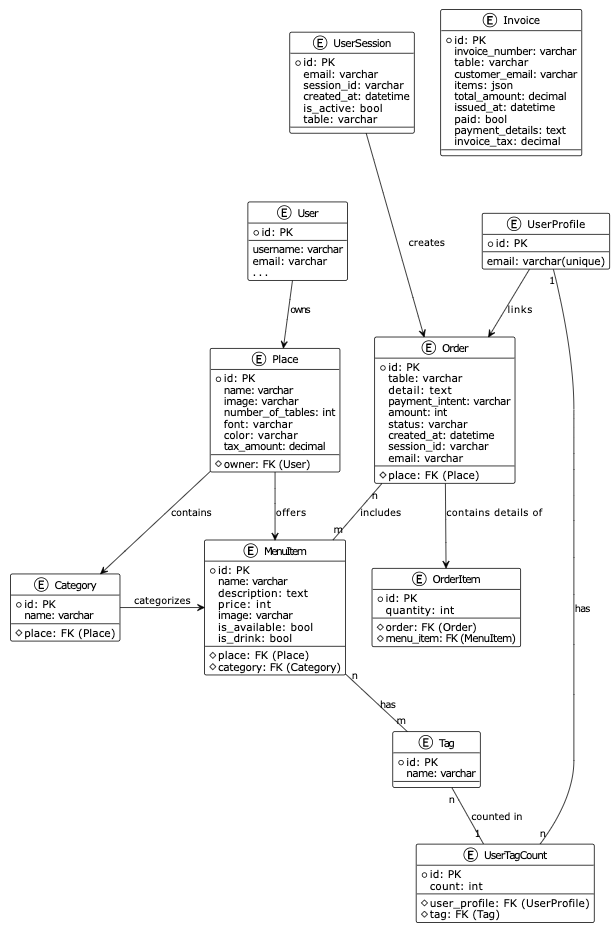
\includegraphics[width=1\textwidth]{images/databasediagram.png}

\subsection{Place}
Represents a restaurant or place that uses the app. It includes details like the owner (linked to the Django \texttt{User} model), name, image, number of tables, and aesthetic customizations (font and color). A new field, \texttt{tax\_amount}, has been added to manage tax calculations.

\subsection{Category}
Organizes menu items into categories (e.g., appetizers, entrees, desserts) for each place. This helps in structuring the menu for easier navigation by the customers.

\subsection{MenuItem}
Details about each menu item, including the place it belongs to, its category, name, description, price, and availability. It also specifies whether the item is a drink and allows for tagging (e.g., vegan, spicy) through a many-to-many relationship with the \texttt{Tag} model.

\subsection{Tag}
Used to label menu items with specific attributes, enhancing the ability to offer personalized recommendations based on customer preferences. Tags are used to describe attributes of food and based on (research) it has been shown that using attributes of food is a good way to recommend food items to customers.

\subsection{UserSession}
Tracks active sessions by customers, including their email, session ID, and table number. It supports functionalities like order tracking and session management. 

\subsection{Order}
Records details of customer orders, including the items ordered (linked through \texttt{OrderItem}), the table and place, payment information, and status. It also tracks the session and customer email.

\subsection{OrderItem}
A through model for the many-to-many relationship between \texttt{Order} and \texttt{MenuItem}, capturing the quantity of each menu item ordered.

\subsection{Invoice}
Manages billing information, including the items ordered, total amount, and payment status. It introduces the \texttt{items} field as a JSON structure to store ordered items, allowing for flexible representation of order details.

\subsection{UserProfile}
Represents a user's profile with a unique email. It is linked to \texttt{Tag} through \texttt{UserTagCount} to track preference metrics.

\subsection{UserTagCount}
Tracks the count of tags associated with a user's orders, facilitating the personalization engine to recommend items based on preferred tags.

% \section{Personalization and Recommendations}
% The schema supports advanced personalization features:
% \begin{itemize}
%     \item \textbf{Personalized Menu Recommendations:} By analyzing a user's order history and preferences (e.g., most ordered tags, preferred price range), the system can recommend menu items that match their taste. This is achieved through methods in the \texttt{UserProfile} model, which calculate preferences based on past orders and tag popularity.
%     \item \textbf{Recommendation Algorithms:} The application uses detailed methods within \texttt{UserProfile} to recommend not only individual food and drink items but also combo meals by creating all possible combinations of recommended food and drink items.
% \end{itemize}

% \section{Key Features and Relationships}
% \begin{itemize}
%     \item The system uses Django's built-in \texttt{User} model for authentication and ownership, linking restaurant places directly to user accounts.
%     \item The \texttt{ForeignKey} and \texttt{ManyToManyField} relationships are utilized extensively to create a network of interconnected entities, enabling complex queries for personalization, order tracking, and session management.
%     \item The application's database design is geared towards enhancing the user experience through features like personalized recommendations, flexible ordering sessions, and detailed order and billing management.
%     \item The use of methods like \texttt{create\_session\_for\_email} in \texttt{UserSession} and recommendation algorithms in \texttt{UserProfile} demonstrate the application's dynamic and user-focused functionality.
% \end{itemize}
% This architecture facilitates a rich, interactive, and personalized user experience in the restaurant management domain, blending traditional e-commerce models with innovative features tailored to the hospitality industry.

\section {Digital Menu Implementation}
QR codes placed on each table serve as the entry point for customers to access the menu and place orders. Upon scanning the QR code with a smartphone, customers are directed to a web interface where they can browse the menu, make selections, and specify their order preferences.
\subsection{Menu Display}
The menu is organized into categories, with each item displaying its name, description, price, and availability. The user interface is designed to be visually appealing and easy to navigate, with a responsive layout that adapts to different screen sizes.
\subsection{Order Placement}
Customers can add items to their order by clicking on the menu items and specifying the quantity. The system tracks the items ordered and the customer's session, allowing for order tracking and billing.
\subsection{Personalized Recommendations}
The application uses the customer's order history and preferences to recommend menu items that match their taste. This is achieved through methods in the \texttt{UserProfile} model, which calculate preferences based on past orders and tag popularity. The algorithm takes into account the most ordered tags and preferred price range to recommend items that align with the customer's preferences.

\section{Reocommender Algorithm}
The recommendation algorithm embedded within the \texttt{UserProfile} model of our restaurant management application is designed to offer personalized menu suggestions to users. It analyzes users' past orders, preferences, and price sensitivity to recommend items that align with their tastes.

\subsection{Possible Implementations}
The recommendation algorithm can be implemented in several ways. Here are some of the considered directions.

\subsection*{Collaborative Filtering}
Collaborative filtering recommends items based on the preferences of similar users. It identifies users with similar tastes and suggests items that they have liked. This method is effective for discovering new items based on the preferences of a user's peers \cite{26} \cite{27}.

\subsection*{Content-Based Filtering}
Content-based filtering uses item features to recommend other items similar to what the user likes, based on their previous actions or explicit feedback. It is based on the idea that if a user likes a particular item, they will also like items that are similar to it. The algorithm uses attributes of the items to recommend other items with similar attributes. User profiles are created based on the items they have interacted with, and recommendations are made based on the similarity between the user profile and the item attributes \cite{29}.

\subsection*{Hybrid Filtering}
Hybrid Filtering combines collaborative and content-based filtering to leverage the strengths of both approaches. By combining the two methods, the system can provide more accurate and diverse recommendations, addressing the limitations of individual techniques \cite{30}. This method is used by web services such as Netflix and Amazon to provide personalized recommendations to users \cite{33}.

\subsection*{Deep Learning Models}
Neural networks can be used to learn complex patterns in user-item interactions, enabling more accurate and personalized recommendations. These models can capture non-linear relationships between users and items, improving the quality of recommendations. However, they require large amounts of data and computational resources \cite{31}.

\subsection*{Stable Matching Algorithms}
Stable matching algorithms can be used to match users with items based on their preferences and constraints. By formulating the recommendation problem as a stable matching problem, the system can generate optimal matches between users and items, ensuring fairness and efficiency \cite{32}. However, this method requires additional feedback from users to determine if it was a good match which can be inconvenient for the user.

\subsection*{Conclusion}
The approach that has been chosen for this implementation is Hybrid Filtering. The system combines collaborative and content-based filtering to provide more accurate and diverse recommendations. While not using the traditional user-to-user collaborative filtering, the system uses the user's past orders and preferences to recommend items that align with their tastes. This way the customer does not need to provide a preference when they first make their order and the recommender system can instead learn from their past orders. This method leverages the strengths of both collaborative and content-based filtering. The algorithm can use the attributes of menu items and user preferences based of their past orders to recommend items that align with the user's taste profile.


\subsection{User Preferences and Order History Analysis}
The algorithm analyses the user's previous orders to deduce their preferences. The algorithm calculates the average price of the items ordered to establish a preferred price range and identifies the most ordered tags to understand the user's food preferences. This information is then used to score and recommend menu items that align with the user's taste.

\subsection{Tag-Based Recommendations}
The algorithm scores menu items based on the user's preferred tags and price sensitivity. The tags represent the attributes of the items, such as vegetarian, healthy, or spicy. By matching the tags of the menu items with the user's preferred tags, the algorithm can recommend items that are likely to appeal to the user. The reason behind the choice to use tags 

\subsection{Price Sensitivity}
The algorithm calculates the user's preferred price range based on their past orders. By analyzing the average price of the items ordered, the system establishes a price range that the user is comfortable with. This information is used to filter out menu items that fall outside the user's price range, ensuring that the recommendations are tailored to the user's budget. The relationship between price and food choice has been highlighted. Research papers \cite{34} and \cite{35} has indicated that a large percentage of the population prioritizes price as the most determining factor in food choice, often opting for cheaper food regardless of its health or environmental impact.

\subsection{Personalized Recommendations}
The recommendation algorithm scores menu items based on the user's preferred tags and price sensitivity. By matching the tags of the menu items with the user's preferred tags and boosting the score if the price of the food item fits within the user's preferred price range, the algorithm can recommend items that are likely to appeal to the user. The algorithm ranks the menu items based on the score, providing personalized recommendations that align with the user's taste profile. It does the same for both food and drink items

\subsection{Combining Recommendations for Combo Meals}
The recommendation algorithm goes a step further by creating all possible combinations of recommended food and drink items to suggest combo meals to the user. By combining the top recommended food and drink items. This would save the customer time when ordering and would also increase the chances of the customer ordering more items. This is a common strategy used by restaurants to increase sales.

\subsection{Example Usage}
\subsection*{Step 1: Determining the Preferred Price Range}

Assume the user has ordered the following items:

\begin{itemize}
    \item Pizza: \$12 (Quantity: 2)
    \item Burger: \$9 (Quantity: 1)
    \item Salad: \$7 (Quantity: 3)
\end{itemize}

\subsection*{Calculation}

\begin{verbatim}
Total spent on Pizza = $12 * 2 = $24
Total spent on Burger = $9 * 1 = $9
Total spent on Salad = $7 * 3 = $21

Total spent = $24 + $9 + $21 = $54
Total quantity of items ordered = 2 + 1 + 3 = 6

Average price per item = Total spent / Total quantity = $54 / 6 = $9
\end{verbatim}

Preferred price range is calculated as ±20 percent of the average price:
\begin{verbatim}
Lower bound = $9 * 0.8 = $7.20
Upper bound = $9 * 1.2 = $10.80
\end{verbatim}

\subsection*{Step 2: Identifying Most Ordered Tags}

Given tags for each item:
\begin{itemize}
    \item Pizza: ["Italian", "Cheese"]
    \item Burger: ["American", "Beef"]
    \item Salad: ["Vegetarian", "Healthy"]
\end{itemize}

The most ordered tags based on quantity are "Vegetarian" and "Healthy".

\subsection*{Step 3: Scoring and Recommending Menu Items}

New menu items to recommend:
\begin{itemize}
    \item Spaghetti: \$8 ["Italian", "Vegetarian"]
    \item Chicken Wrap: \$10 ["Healthy", "Chicken"]
    \item Fish Tacos: \$11 ["Seafood"]
    \item Veggie Burger: \$9 ["Vegetarian", "American"]
\end{itemize}

\subsection*{Scoring}

Spaghetti scores high for matching "Vegetarian" and being within the price range.
Chicken Wrap scores for "Healthy" and being within the price range.
Fish Tacos score lower due to being outside the price range and no matching tags.
Veggie Burger scores for "Vegetarian" and being within the price range.


\subsection*{Results}

Based on the scoring, the recommended items in order are:
\begin{enumerate}
    \item Spaghetti
    \item Chicken Wrap
    \item Veggie Burger
\end{enumerate}

\section{Flexible Bill Sharing}

This section outlines the systematic steps taken to design, implement, and evaluate this bill splitting implementation.

\subsection{Design Considerations}
A primary focus was to ensure an intuitive and hassle-free interaction with the bill-sharing feature, allowing customers to easily choose between individual payments or sharing the bill with others. The feature needed to accurately calculate and split the bill according to the specific orders and preferences of the diners, providing flexibility in how the bill could be shared. The system has to manage individual and group ordering, allowing customers to order individually or as a group, while ensuring accurate tracking of orders and payments.

\subsection*{Possible Implementations}


\subsection{Implementation}
\begin{itemize}
    \item \textbf{Order Placement via individual Sessions}: When customers scan the QR code at their table, they have the option to create an individual ordering session by entering their email address. This process ensures that each diner's selections are tracked separately, even though they are physically sitting at the same table.
    \item \textbf{Joining Sessions for Shared Billing}: The application provides an option for customers to join a session created by another diner at the same table. This feature is particularly useful for groups who want to combine their orders into a single bill, allowing easy payment splitting without the need for manual calculations or multiple transactions.
    \item \textbf{Separate Payments or Single Payment}: At the end of the meal, the group can decide whether to pay separately or together. If they opt for individual payments, each diner pays only for their ordered items. For a shared bill, the total cost is evenly divided among the participants in the joined session, or the payment can be split according to the specific items each person ordered, depending on the application's capabilities and settings.
\end{itemize}

\section{Admin Panel}
\subsection{Features}
\begin{itemize}
    \item \textbf{Order Tracking}: Provides real-time tracking of customer orders, allowing staff to monitor and manage orders efficiently. This feature allows the adminstrator to keep track of which tables are occupied, the time since the last order, and the status of each order.
    \item \textbf{Billing and Invoice Management}: The adminstrator can manage billing and invoices, for each table and would be able to see all the separate sessions that are on that table. This feature also allows the adminstrator to view and manage the billing and invoices for each table, including the ability to split bills and track payments. All paid and unpaid invoices are stored, allowing the adminstrator to view and manage them as needed. The invoices are designed to work with carbon printers as well.
    \item \textbf{Sales Analysis}: The adminstrator can view sales data such as daily, weekly and monthly sales. The adminstrator can also view the most popular items and the least popular items. This feature also displays the peak hours of the day which along side with the popular items can be used to make decisions on inventory.
    \item \textbf{Global Settings}: The adminstrator can manage global settings such as tax rates, menu themes and fonts. They can also change the name of the restaurant and the logo.
\end{itemize}

\section{Kitchen Display System}
\subsection{Features}
\begin{itemize}
    \item \textbf{Real-time Order Display}: The kitchen display system provides a real-time display of incoming orders, allowing kitchen staff to prepare and manage orders. This feature allows the kitchen staff to view the orders as they come in, and mark them as in progress or completed.
    \item \textbf{Separate Displays}: The system can display orders for different stations on separate screens, allowing staff to focus on their specific tasks. This feature allows the kitchen staff to view the orders that are relevant to their station, and manage them accordingly. Such as the bar which would only display drink orders.
    \item \textbf{Time Warnings:} When the order time exceeds 15 minutes, the order would turn yellow and when it exceeds 25 minutes, the order would turn red. This feature allows the kitchen staff to prioritize orders based on their urgency.
\end{itemize}

\section{Floor Staff Display}
\subsection{Features}
\begin{itemize}
    \item \textbf{Order Tracking}: The orders that have been prepared by the kitchen would be displayed.
    \item \textbf{Table Numbers}: The table numbers of the orders would be displayed.
    \item \textbf{Update Status}: Once the order has been served, the floor staff would be able to update the status of the order as served.
\end{itemize}

\section{Menu Management}
\subsection{Features}
\begin{itemize}
    \item \textbf{Add New Items}: The system should allow restaurant staff to add new items to the menu, including specifying the name, description, price, category, tags which will be used for the recommendation algorithm, and availability of the item. This feature allows the restaurant staff to add new items to the menu as needed, and specify the details of each item.
    \item \textbf{Update Items}: The system should allow restaurant staff to update existing items on the menu, including changing the name, description, price, category, tags, and availability of the item. This feature allows the restaurant staff to update the details of existing items on the menu as needed.
    \item \textbf{Remove Items}: The system should allow restaurant staff to remove items from the menu that are no longer available. This feature allows the restaurant staff to remove items from the menu that are no longer available or have been discontinued.
    \item \textbf{Create Categories}: The system should allow restaurant staff to create new categories for the menu, and assign items to specific categories. This feature allows the restaurant staff to organize the menu into different categories, making it easier for customers to navigate and find items.
    \item \textbf{Manage Tags}: The system should allow restaurant staff to manage tags for each item, specifying the attributes of the item such as vegan, spicy, or gluten-free. This feature allows the restaurant staff to tag items with specific attributes, which will be used for the recommendation algorithm.
\end{itemize}

\chapter{Project Management}

\chapter{Evaluation}
\section{Technical Evaluation}
API testing were carried out to the Django backend to measure the performance of the system. The API testing was done using Postman. The custom API requests were made through Postman and the requests have been designed to mimic real world use.

\subsection{API Testing}
Both the server and the database are needed to be tested with multiple requests per second. Specifically the Ordering API was tested in this experiment. The reason to this is to test how the server would handle multipe order requests at the same time. Postman was used to send multiple POST requests to the server because the platform allows tests to be written in JavaScript and run in the Postman environment. Provided with the correct body and headers in the API call, every request had to return a 200 response code. The treshold for any response time is 200ms to maintain a responsive system. The tests are separated between POST requests and GET requests. The POST requests are used to send data and the GET requests are used to retrieve from the database.

\subsection{POST Request Testing}
Some of the most demanding POST requests were used in testing and these chosen POST requests are the ones that are most likely to be used in a real world scenario and will have the most impact to the system efficiency and user experience. The specific POST request that was tested is the create order request (http://localhost:8000/api/create-payment-intent/). This POST API call is responsible for creating a new order in the database. The request body is a JSON object that contains the order details such as the items, the total amount, the customer details and the payment method.





\chapter{Discussion}

% Conclusion
\chapter{Conclusion}
% Add your conclusion chapter here
\chapter{Appendix}
\include{chapters/appendix}
% References
\begin{thebibliography}{}
    \bibitem{1} R. Paul, R. R. Bhandopia, D. R. Patil, J. D. Raut, and A. D. Gotmare, ‘An Efficient Digital Ordering System for Restaurant’, Ijresm.com. [Online]. Available: \url{https://www.ijresm.com/Vol.3_2020/Vol3_Iss3_March20/IJRESM_V3_I3_103.pdf}. [Accessed: 17-Mar-2024].

    \bibitem{2} ‘(PDF) Smart QR-based Restaurant Dine-in System with Sales Analysis’, ResearchGate. [Online]. Available: \url {https://www.researchgate.net/publication/360414606_Smart_QR-based_Restaurant_Dine-in_System_with_Sales_Analysis/fulltext/627a7d2b2f9ccf58eb3d5475/Smart-QR-based-Restaurant-Dine-in-System-with-Sales-Analysis.pdf}. [Accessed: 17-Mar-2024].

    \bibitem{3}D. Carcache and R. E, “Automated Services Order System,” prcrepository.org, 2013, Accessed: Mar. 17, 2024. [Online]. Available: \url {https://prcrepository.org/xmlui/handle/20.500.12475/836?show=full}

    \bibitem{4} K. Dhiman, “Online Food Ordering Management System,” International Journal for Research in Applied Science and Engineering Technology, vol. 9, no. VII, pp. 2096–2107, Jul. 2021, doi: {https://doi.org/10.22214/ijraset.2021.36835}.
    
    \bibitem{5} ‘(PDF) Customer Acceptance of QR Menu Ordering System in Luxury Restaurants. A study of Xi’an, China’, ResearchGate. [Online]. Available: \url{https://www.researchgate.net/profile/Anshul-Garg-4/publication 377586294_Customer_Acceptance_of_QR_Menu_Ordering_System_in_Luxury_Restaurants_A_study_of_Xi'an_China/links/65ae68e29ce29c458b939be6/Customer-Acceptance-of-QR-Menu-Ordering-System-in-Luxury-Restaurants-A-study-of-Xian-China.pdf}. [Accessed: 17-Mar-2024].

    \bibitem{6}
    B. Shadaksharappa, Kotrachaithanya, and D. Kumar, “FOOD HUB A Model for Ordering In Restaurant Based On Qr Code Without Presence Of A Waiter At The Table,” International Journal of Engineering Research in Computer Science and Engineering (IJERCSE), vol. 5, no. 5, pp. 2394–2320, 2018, Available: \url{https://www.technoarete.org/common_abstract/pdf/IJERCSE/v5/i5/Ext_34756.pdf}.

    \bibitem{7}
    E. E. Abel and E. Obeten, ‘Restaurant customer self-ordering system: A solution to reduce customer/guest waiting time at the Point of sale’, Ijcaonline.org. [Online]. Available: \url{https://research.ijcaonline.org/volume111/number11/pxc3901332.pdf}. [Accessed: 17-Mar-2024].


    \bibitem{8} Toast, Inc., "Toast: Restaurant Point of Sale and Management System," [Online]. Available: \url{https://pos.toasttab.com/}. [Accessed: Mar. 17, 2024].

    \bibitem{9} Square, Inc., "Square: Solutions For Your Small, Medium and Large Business," [Online]. Available: \url{https://squareup.com/}. [Accessed: Mar. 17, 2024].

    \bibitem{10} Zuppler, "Zuppler: Online Ordering System for Restaurants," [Online]. Available: \url{https://www.zuppler.com/}. [Accessed: Mar. 17, 2024].

    \bibitem{11} TouchBistro Inc., "TouchBistro: iPad POS System for Restaurants, Bars, and More," [Online]. Available: \url{https://www.touchbistro.com/}. [Accessed: Mar. 17, 2024].

    \bibitem{12} Bbot, "Bbot: Contactless Order and Pay," [Online]. Available: \url{https://www.bbot.menu/}. [Accessed: Mar. 17, 2024].

    \bibitem{13} Menufy, "Menufy: Online Ordering for Restaurants," [Online]. Available: \url{https://www.menufy.com/}. [Accessed: Mar. 17, 2024].

    \bibitem{14} Future Ordering, "Future Ordering: Digital Ordering Solutions," [Online]. Available: \url{https://www.futureordering.com/}. [Accessed: Mar. 17, 2024].

    \bibitem{15} React Team, "React – A JavaScript library for building user interfaces," React. [Online]. Available: \url{https://reactjs.org/}. [Accessed: Mar. 17, 2024].

    \bibitem{16} Django Software Foundation, "Django: The web framework for perfectionists with deadlines," Django. [Online]. Available: \url{https://www.djangoproject.com/}. [Accessed: Mar. 17, 2024].

    \bibitem{17} SQLite, "SQLite Home Page," SQLite. [Online]. Available: \url{https://sqlite.org/index.html}. [Accessed: Mar. 17, 2024].

    \bibitem{18} Axios, "Axios GitHub repository," GitHub. [Online]. Available: \url{https://github.com/axios/axios}. [Accessed: Mar. 17, 2024].

    \bibitem{19} D. Abramov and A. Clark, "Introducing Hooks," React, Oct. 25, 2018. [Online]. Available: \url{https://reactjs.org/docs/hooks-intro.html}. [Accessed: Mar. 17, 2024].

    \bibitem{20} T. Otwell, "Laravel: The PHP Framework For Web Artisans," Laravel. [Online]. Available: \url{https://laravel.com}. [Note: Replace with Django REST Framework if specific documentation is available]. [Accessed: Mar. 17, 2024].

    \bibitem{21} React Router, "React Router: Declarative Routing for React.js," ReactRouter. [Online]. Available: \url{https://reactrouter.com/}. [Accessed: Mar. 17, 2024].

    \bibitem{22} Bulma, "Bulma: a modern CSS framework based on Flexbox," Bulma. [Online]. Available: \url{https://bulma.io/}. [Accessed: Mar. 17, 2024].

    \bibitem{23} AWS, "Amazon Web Services (AWS) - Cloud Computing Services," Amazon. [Online]. Available: \url{https://aws.amazon.com/}. [Accessed: Mar. 17, 2024].

    \bibitem{24} Heroku, "Heroku: Cloud Application Platform," Heroku. [Online]. Available: \url{https://www.heroku.com/}. [Accessed: Mar. 17, 2024].

    \bibitem{25} Railway, "Railway: Infrastructure for modern applications," Railway. [Online]. Available: \url{https://railway.app/}. [Accessed: Mar. 17, 2024].

    \bibitem{26}Real Python, “Build a Recommendation Engine With Collaborative Filtering,” Realpython.com, Jul. 10, 2019. https://realpython.com/build-recommendation-engine-collaborative-filtering/ (accessed Mar. 22, 2024)

    \bibitem{27}“What Is Collaborative Filtering: A Simple Introduction,” Built In, 2019. https://builtin.com/data-science/collaborative-filtering-recommender-system (accessed Mar. 22, 2024).

    \bibitem{28} Shivam Baldha, “Introduction to Collaborative Filtering,” Analytics Vidhya, Feb. 25, 2022. https://www.analyticsvidhya.com/blog/2022/02/introduction-to-collaborative-filtering/ (accessed Mar. 22, 2024).

    \bibitem{29} A. Roy, “Introduction To Recommender Systems- 1: Content-Based Filtering And Collaborative Filtering,” Medium, Jul. 29, 2020. https://towardsdatascience.com/introduction-to-recommender-systems-1-971bd274f421 (accessed Mar. 22, 2024).

    \bibitem{30} Hybrid Recommender Systems, “Hybrid Recommender Systems | Saturn Cloud,” Saturncloud.io, Feb. 23, 2023. https://saturncloud.io/glossary/hybrid-recommendation-system/ (accessed Mar. 22, 2024).

    \bibitem{31} Sciforce, “Deep Learning Based Recommender Systems - Sciforce - Medium,” Medium, Apr. 30, 2021. https://medium.com/sciforce/deep-learning-based-recommender-systems-b61a5ddd5456 (accessed Mar. 22, 2024).

    \bibitem{32} Krishnakanth Naik Jarapala, “Understanding Gale-Shapley (Stable Matching ) Algorithm and its Time Complexity,” Medium, Jan. 31, 2023. https://medium.com/aiskunks/understanding-gale-shapley-stable-matching-algorithm-and-its-time-complexity-4b814ee2642 (accessed Mar. 22, 2024).

    \bibitem{33} “How Netflix’s Recommendations System Works,” Help Center, 2024. https://help.netflix.com/en/node/100639 (accessed Mar. 23, 2024).

    \bibitem{34} M. Geuens, “Research on Influencing Factors of Food Choice and Food Consumption,” Foods, vol. 12, no. 6, pp. 1306–1306, Mar. 2023, doi: https://doi.org/10.3390/foods12061306.

    \bibitem{35} Ingrid H.M. Steenhuis, W. E. Waterlander, and Anika de Mul, “Consumer food choices: the role of price and pricing strategies,” Public Health Nutrition, vol. 14, no. 12, pp. 2220–2226, Jul. 2011, doi: https://doi.org/10.1017/s1368980011001637.
    ‌
    ‌
    ‌
    ‌
    ‌
    ‌
    ‌
    ‌
    ‌
    ‌







    

\end{thebibliography}

\end{document}